%%+++++++++++++++++++++++++++++++++++++%%
%%         Final Version  6/14/95      %%
%%+++++++++++++++++++++++++++++++++++++%%
\documentclass[12pt]{article}
\textheight = 8.6in
\textwidth = 6.2in
\topmargin = -.5in
\oddsidemargin = 0.08in
\evensidemargin = 0.08in
%\usepackage{fancyhdr}
%\pagestyle{fancy}
%\rfoot{\thepage}
\setlength{\jot}{10.0 pt}
\setlength{\parskip}{2.0ex}
\setlength{\footskip}{65pt}

\usepackage{graphicx}
\usepackage{subfigure}
\usepackage{placeins}
\usepackage{afterpage}
\usepackage{amsmath}
\usepackage{empheq}
\usepackage[most]{tcolorbox}
\newtcbox{\mymath}[1][]{%
    nobeforeafter, math upper, tcbox raise base,
    enhanced, colframe=white!20!black ,
    colback=blue!30!red!30!white, boxrule=1pt,
    #1}
\usepackage{xcolor}
\definecolor{myblue}{RGB}{0, 0, 180}   %Numbers are integers from 0 to 255, smaller is closer to black
\definecolor{grey}{RGB}{200, 200, 200}   %Numbers are integers from 0 to 255, smaller is closer to black
\definecolor{mygreen}{RGB}{0, 100, 0}   %Numbers are integers from 0 to 255, smaller is closer to black
\definecolor{myred}{RGB}{120, 0, 0}   %Numbers are integers from 0 to 255, smaller is closer to black

\begin{document}

\begin{flushright} {\color{blue} Chapter 3, Lecture 3} \end{flushright}
\begin{flushleft}

\subsubsection*{\color{myblue} \bf Separation of Variables: Laplace's equation in Cartesian coordinates}

Separation of variables is a technique for finding a solution to a partial differential equation (such as Laplace's equation).  In this method, a solution is postulated that is a product of functions, each of these functions in only one of the independent variables.  This product solution is substituted into the partial differential equation, in hopes of going to two or three ordinary differential equations, each one in terms of only one of the independent variables.  If this can be done, then each ordinary differential equation is considered separately to find a functional form of the solution for this independent variable.  Laplace's equation is solvable using the separation of variables technique.

Consider the simplest case, the two-dimensional Laplace equation in cartesian coordinates:

\begin{equation*}
\begin{aligned}
& \nabla^{2}V(x,y) = 0 \\[6pt]
& \frac{\partial^{2} V(x,y)}{\partial x^{2}} + \frac{\partial^{2} V(x,y)}{\partial y^{2}} = 0
\end{aligned}
\end{equation*}

Write $V(x,y)$ as a product of functions, each dependent on only one of the independent variables, $V(x,y)=\mathcal{X}(x)\mathcal{Y}(y)$.  Substituting this product of functions for $V(x,y)$ in Laplace's equation,

\begin{align}
& \frac{\partial^{2} \mathcal{X}(x)\mathcal{Y}(y)}{\partial x^{2}} + \frac{\partial^{2} \mathcal{X}(x)\mathcal{Y}(y)}{\partial y^{2}} = 0 \notag \\[6pt]
&  \mathcal{Y}(y)\frac{\partial^{2} \mathcal{X}(x)}{\partial x^{2}} + \mathcal{X}(x)\frac{\partial^{2} \mathcal{Y}(y)}{\partial y^{2}} = 0 \label{eq:productthere}
\end{align}

Now divide both sides of Eq.~\ref{eq:productthere} by $\mathcal{X}(x)\mathcal{Y}(y)$:

\begin{equation}
\frac{1}{\mathcal{X}(x)}\frac{\partial^{2} \mathcal{X}(x)}{\partial x^{2}} + \frac{1}{\mathcal{Y}(y)}\frac{\partial^{2} \mathcal{Y}(y)}{\partial y^{2}} = 0
\label{eq:independentterms}
\end{equation}

The first term of Eq.~\ref{eq:independentterms} has only $x$-dependence, while the second term of Eq.~\ref{eq:independentterms} has only $y$-dependence.  Each term must be a constant.  To see this, suppose the second term is fixed ($y$ is fixed).  The first term must be equal and opposite to the second term, or else the terms would not sum to zero as required.  For the first term to be equal and opposite the second term \textit{no matter the value of x}, both terms must be (equal and opposite) constants!  That is,

\begin{eqnarray}
& & \frac{1}{\mathcal{X}(x)}\frac{\partial^{2} \mathcal{X}(x)}{\partial x^{2}} + \frac{1}{\mathcal{Y}(y)}\frac{\partial^{2} \mathcal{Y}(y)}{\partial y^{2}} = 0  \label{eq:separated} \\[6pt]
& & K^{2} - K^{2} = 0 \hspace{1.8in} \rightarrow \hspace{.2in} \text{\color{mygreen} where $K$ is a constant} \nonumber
\end{eqnarray}

A squared constant, $K^{2}$, was chosen for convenience.  Since the constant is unknown at this point, the exact form of the constant doesn't affect the final solution.  The form of the constant does make solution of the ordinary differential equations more or less convenient.  Then each term of Eq.~\ref{eq:separated} may be set equal to its assigned constant value:
\begin{align}
& \frac{1}{\mathcal{X}(x)}\frac{d^{2} \mathcal{X}(x)}{dx^{2}} = K^{2} \label{eq:xeq} \\[6pt]
& \frac{1}{\mathcal{Y}(y)}\frac{d^{2} \mathcal{Y}(y)}{dy^{2}} = -K^{2} \label{eq:yeq}
\end{align}

Notice that equations \ref{eq:xeq} and \ref{eq:yeq} are now ordinary differential equations.  Since $\mathcal{X}(x)$ is a function only of $x$, and $\mathcal{Y}(y)$ is a function only of $y$, total derivatives may be used instead of partial derivatives.  Rewriting Eq.\ref{eq:yeq}, we see that it has the form of the classic harmonic oscillator equation:

\begin{align}
& \frac{1}{ \mathcal{Y}(y) }\frac{d^{2} \mathcal{Y}(y)}{dy^{2}} = -K^{2} \notag \\[6pt]
& \frac{d^{2} \mathcal{Y}(y)}{dy^{2}} = -K^{2} \,\mathcal{Y}(y) \notag \\[6pt]
& \frac{d^{2} \mathcal{Y}(y)}{dy^{2}} + K^{2} \,\mathcal{Y}(y) \notag = 0
\end{align}

The general solution of the harmonic oscillator equation is known,

\begin{equation}
\mathcal{Y}(y) = A \cos{(Ky)} + B \sin{(Ky)}
\label{eq:singleharmonic}
\end{equation}

On the other hand, Eq.\ref{eq:xeq} does \textit{not} look like the harmonic oscillator equation, because there is a \textit{positive} constant on the RHS:

\begin{align}
& \frac{1}{ \mathcal{X}(x) }\frac{d^{2} \mathcal{X}(x)}{dx^{2}} = K^{2} \notag \\[6pt]
& \frac{d^{2} \mathcal{X}(x)}{dx^{2}} = K^{2} \,\mathcal{X}(x) \notag \\[6pt]
& \frac{d^{2} \mathcal{X}(x)}{dx^{2}} - K^{2} \,\mathcal{X}(x) \notag = 0
\end{align}

As you can verify, the general solution in this case has exponential functions:

\begin{equation}
\mathcal{X}(x) = A e^{(-Kx)} + B e^{(+Kx)}
\label{eq:singleexp}
\end{equation}

You may have a few questions at this point.  We could have reversed the assignment of constants so that the equation for $\mathcal{X}(x)$ would have been the harmonic oscillator equation, whereas the equation for $\mathcal{Y}(y)$ had the exponential solutions.  Also, our choice of constant $K$ was arbitrary, we could have picked some other constant, say $\Lambda$.  These things are dependent on the physical situation to which  Laplace's equation is being applied; at the end of the day the solution must obey the boundary conditions of the problem.

Whether parameter $x$ or $y$ is assigned harmonic behavior can usually be determined with a little intuition.  If your 'guess' is incorrect, it will be hard to match the boundary conditions.  As far as the constant $K$ goes, more than one constant value might satisfy the boundary conditions.  So, to be on the safe side, choose all possible constants!  For example, in the case above, instead of writing Eq.~\ref{eq:singleharmonic}, write the general expression,

\begin{equation*}
\mathcal{Y}(y) = \sum_{\text{n}=0}^{\infty} a_{n} \cos{(k_{n}y)} + b_{n} \sin{(k_{n}y)}
%\label{eq:allharmonics}
\end{equation*}

Similarly, replace Eq.~\ref{eq:singleexp} with the following,

\begin{equation*}
\mathcal{X}(x) = \sum_{n=0}^{\infty} c_{n}e^{(-k_{n}x)} + d_{n}e^{(k_{n}x)}
%\label{eq:allexp}
\end{equation*}

What the constants actually are, and how many of them are needed, will be determined later when the boundary conditions are applied.  In summary, the total general solution for the potential, $V(x,y)$ (for this two-dimensional Cartesian case we have been discussing) before applying boundary conditions is as follows:

\begin{eqnarray}
V(x,y) & = & \mathcal{X}(x)\mathcal{Y}(y) \nonumber \\
& = & \sum_{n=0}^{\infty} \left( c_{n}e^{(-k_{n}x)} + d_{n}e^{(k_{n}x)} \right) \left( a_{n} \cos{(k_{n}y)} + b_{n} \sin{(k_{n}y)} \right)
\label{eq:gen2Dcartslan}
\end{eqnarray}

Now let's go back to the question as to whether the positive or negative constant should be assigned to the first term of the partial differential equation (Eq~\ref{eq:separated}).  To illustrate, take the example of finding the potential in an enclosed space that is rectangular in cross-section, but 'infinite' in the third dimension.  The lack of boundary in the third dimension makes this a two dimensional problem.  The rectangular shape makes cartesian geometry suitable for this problem.  

Note that this shape has practical applications; as you will find out later when you study dynamics, this rectangular 2D shape is used to guide electromagnetic waves.  In order to have a problem suitable for statics, one side of the rectangular boundary must have a non-zero voltage, otherwise the voltage everywhere inside would be zero (not a very interesting situation).  In the dynamics case, the physics is described by the wave equation instead of Laplace's equation, and so in the dynamics case all sides may be at zero volts and still have a propagating solution.

\begin{figure}[h]
\begin{center}
\subfigure[waveguide section]{
   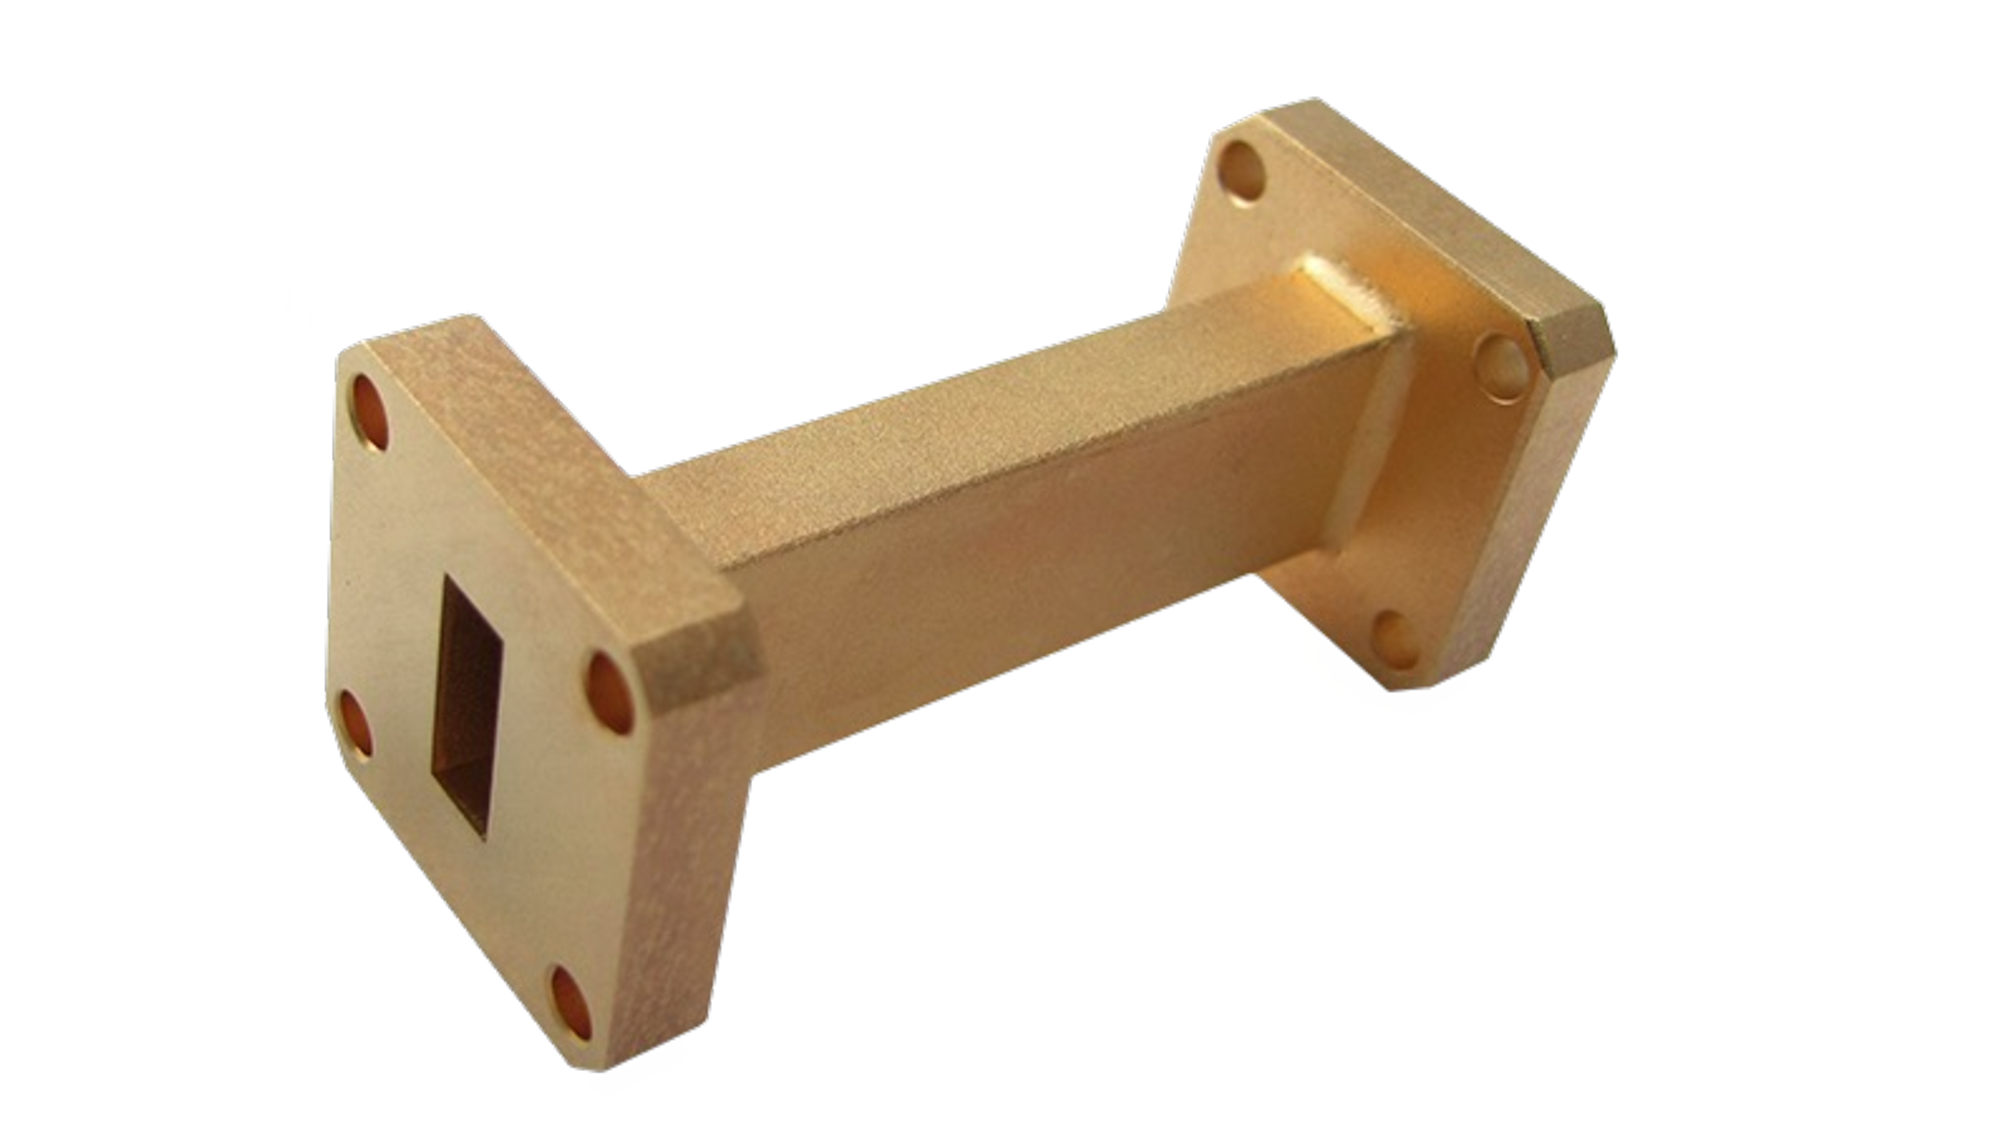
\includegraphics[trim=2cm 0cm 2cm 2cm, clip=true, width=0.42\columnwidth]{waveguide_section.pdf}
   \label{fig:section}
 }
\hspace{0.1in}
\subfigure[FNAL Linac with waveguides]{
   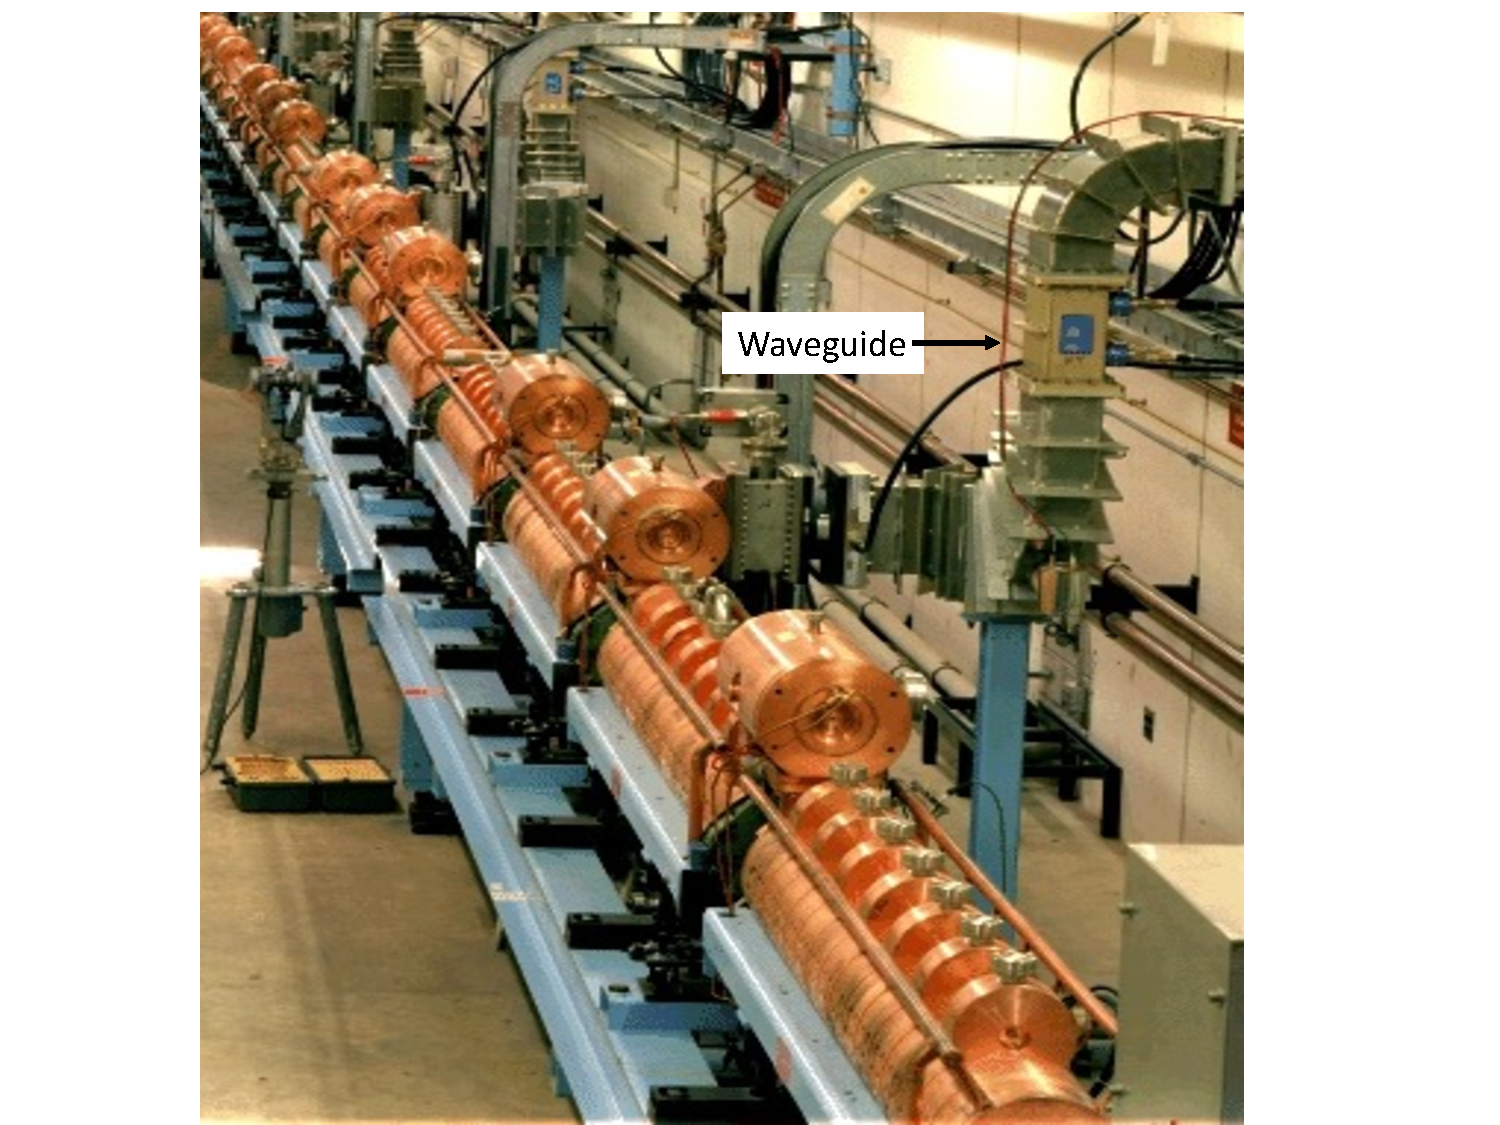
\includegraphics[trim=2cm 0cm 2cm 0cm, clip=true, width=0.47\columnwidth]{waveguide.pdf}
   \label{fig:rightside}
 }
\end{center}
\caption{\small Left: Image taken from $\langle$https://www.hasco-inc.com/millimeterwave/wr-42-millimeter-waveguide-straight-section-2-inch-18-ghz-to-26-5-ghz/$\rangle$, from HASCO vendor site.  Right: Waveguides used to transport electromagnetic power to Fermilab Linac. \textit{Courtesy Fermilab Visual Services.}}
\label{fig:realguides}
\end{figure}

Getting back to the situation at hand: consider the situations of Fig.~\ref{fig:staticguide}, here there are three sides held at zero volts and one 'hot' side held at $V_{0}$ volts.  In Fig.~\ref{fig:topside}, the top side at $y=a$ is held at $V_{0}$ volts while the other three sides are grounded.  In Fig.~\ref{fig:rightside}, the right side at $x=b$ is held at $V_{0}$ volts while the other three sides are grounded.

\begin{figure}[h]
\begin{center}
\subfigure[top side 'hot']{
   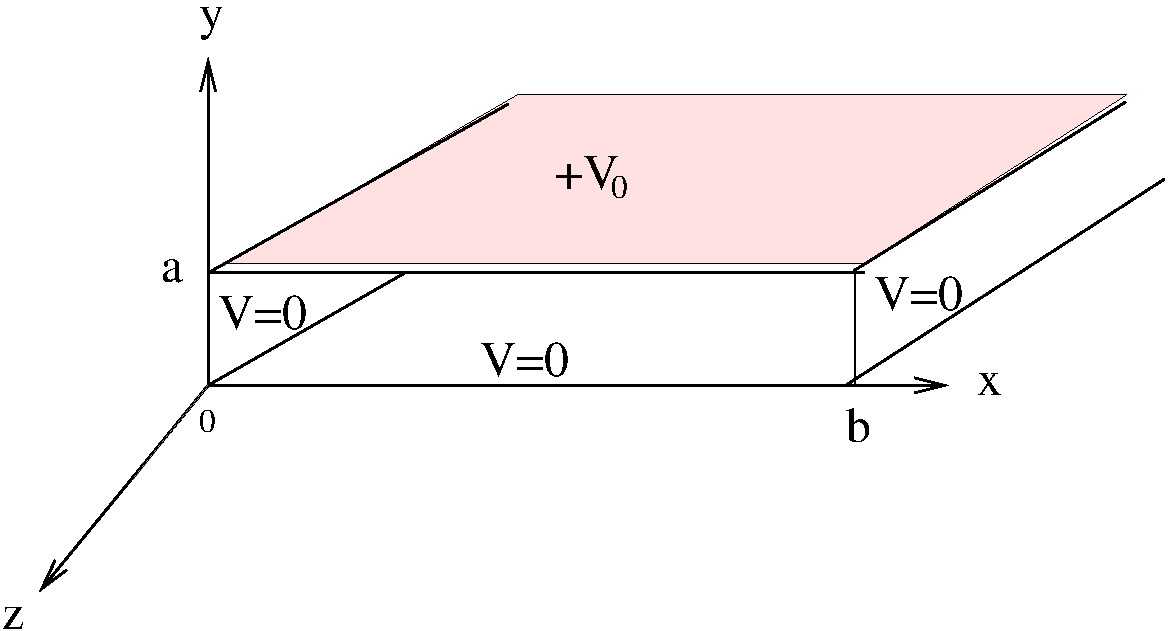
\includegraphics[width=0.40\columnwidth]{anotherguide.pdf}
   \label{fig:topside}
 }
\hspace{0.2in}
\subfigure[right side 'hot']{
   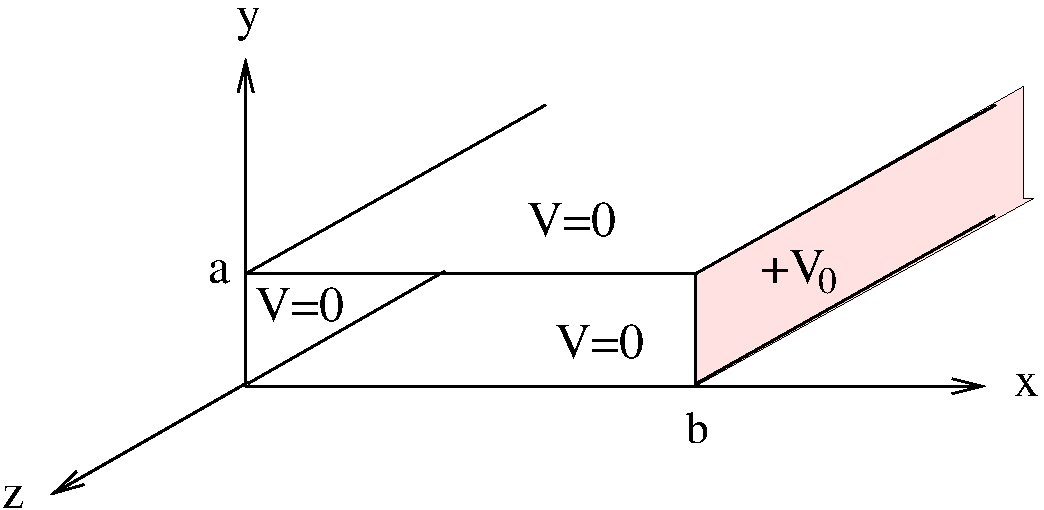
\includegraphics[width=0.40\columnwidth]{staticguide.pdf}
   \label{fig:rightside}
 }
\end{center}
\caption{\small A long pipe of rectangular cross-section, the boundaries of the interior space are the four sides.  All sides except one are grounded (have zero voltage).  Left: the top side is held at +$V_{0}$ volts, all other sides are grounded.  Right: the right side is held at +$V_{0}$ volts, all other sides are grounded.  Assume there are small insulating gaps between any two sides; this allows one 'hot' side.}
\label{fig:staticguide}
\end{figure}
 
Consider the case of Fig.~\ref{fig:topside}, the voltage is zero at the boundaries $x=0$ and $x=b$ requiring that  whatever the functional variation in $\mathcal{X}(x)$, it must go to zero at those two $x$-locations.  Sinusoidal functions have many nodes, while exponential functions (or their combinations) do not have more than one, so the equation for $\mathcal{X}(x)$ must be the harmonic equation in this case.   The equation with exponential solutions will work for $\mathcal{Y}(y)$ for the case shown in Fig.~\ref{fig:topside}, because the boundary at $y=a$ has a non-zero voltage, leaving only one zero at $y=0$ to fit with the function.  The same arguments hold (but applied in reverse) for the case of Fig.~\ref{fig:rightside}.  Here, $\mathcal{Y}(y)$ must be the sinusoidal function.

Suppose we have the case of Fig.~\ref{fig:rightside}; the general solution given by Eq.~\ref{eq:gen2Dcartslan} is appropriate for this case.  The remaining task is to find the as yet undetermined coefficients.  These are found using the boundary conditions, so the first thing to do is explicitly state them.  There are four boundaries, so there must be four Boundary Conditions (B.C.).  These are (for this example):
\begin{itemize}
\item[(1)] $V=0$ at $x=0$
\item[(2)] $V=V_{0}$ at $x=b$
\item[(3)] $V=0$ at $y=0$
\item[(4)] $V=0$ at $y=a$
\end{itemize}

The second boundary condition has the specific voltage that is generating the potential internal to the guide.  Thus, B.C. (2) will be applied last, at which point we'll make use of the orthogonality of sinusoidal functions.  Let's start by applying B.C. (1) to Eq.~\ref{eq:gen2Dcartslan},

\begin{eqnarray*}
V(0,y) & = & \mathcal{X}(0)\mathcal{Y}(y) \\
 0 & = & \sum_{n=0}^{\infty} \left( c_{n}e^{(-k_{n}0)} + d_{n}e^{(k_{n}0)} \right)\mathcal{Y}(y) \\
 0 & = & \sum_{n=0}^{\infty} \left( c_{n} + d_{n} \right) \mathcal{Y}(y) \hspace{.5in} \longrightarrow \hspace{.5in} d_{n} = -c_{n} 
%\label{eq:gen2Dcartslan}
\end{eqnarray*}

Applying B.C. (3) to Eq.~\ref{eq:gen2Dcartslan},

\begin{eqnarray*}
V(x,0) & = & \mathcal{X}(x)\mathcal{Y}(0) \\
0 & = & \sum_{n=0}^{\infty} \mathcal{X}(x) \left( a_{n} \cos{(k_{n}0)} + b_{n} \sin{(k_{n}0)} \right) \\
0 & = & \sum_{n=0}^{\infty} \mathcal{X}(x) a_{n} \hspace{.5in} \longrightarrow \hspace{.5in} a_{n} = 0 
\end{eqnarray*}

Applying B.C. (4) with $a_{n}=0$ to Eq.~\ref{eq:gen2Dcartslan},

\begin{eqnarray*}
V(x,a) & = & \mathcal{X}(x)\mathcal{Y}(a) \nonumber \\
0 & = & \sum_{n=0}^{\infty} \mathcal{X}(x) b_{n} \sin{(k_{n}a)} \hspace{.5in} \longrightarrow \hspace{.5in}  b_{n} \sin{(k_{n}a)} = 0
\end{eqnarray*}

Since $b_{n} \sin{(k_{n}a)}=0$, either $b_{n}=0$, or $k_{n}a=n\pi$ (making the sine function vanish at location $a$).  It cannot be that $b_{n}=0$, because then the voltage inside the guide would be zero everywhere, which cannot be true.  Solutions to Laplace's equations are smooth functions, and the voltage at $x=b$ is \textit{not} zero.  Therefore, $k_{n}a=n\pi$, or $k_{n}=n\pi/a$.

Then,
\begin{eqnarray*}
V(x,y) & = & \sum_{n=0}^{\infty} c_{n}\left( e^{-k_{n}x}-e^{+k_{n}x} \right) b_{n} \sin{(k_{n}y)}\\
          & = & \sum_{n=0}^{\infty} 2c_{n}b_{n}\sinh{ \left(\frac{n\pi x}{a}\right) }\sin{ \left(\frac{n\pi y}{a}\right) } \\
          & = & \sum_{n=0}^{\infty} A_{n}\sinh{ \left(\frac{n\pi x}{a}\right) }\sin{ \left(\frac{n\pi y}{a}\right) } 
\end{eqnarray*}
where the arbitrary constants have been absorbed into a new arbitrary constant, $A_{n}=2c_{n}b_{n}$.

Now the final step is to use B.C. (2) and the orthogonality condition to find specific values for the arbitrary constants $A_{n}$.  (That is for $A_{1}$, $A_{2}$, $A_{3}$, $\ldots$).

\subsubsection*{\color{myblue} Using orthogonal functions to find undetermined coefficients}

The solution so far is given by,

\[
V(x,y) = \sum_{n=0}^{\infty} A_{n}\sinh{ \left(\frac{n\pi x}{a}\right) }\sin{ \left(\frac{n\pi y}{a}\right) } 
\]
 
Apply the last boundary condition ($V=V_{0}$ at $x=b$),

\begin{eqnarray}
\begin{aligned}
& V_{0} = \sum_{n=0}^{\infty} A_{n}\sinh{\left(\frac{n\pi b}{a}\right)}\sin{\left(\frac{n\pi y}{a}\right)} \\
& = A_{1}\sinh{\left(\frac{\pi b}{a}\right)}\sin{\left(\frac{\pi y}{a}\right)} + A_{2}\sinh{\left(\frac{2\pi b}{a}\right)}\sin{\left(\frac{2\pi y}{a}\right)} + A_{3}\sinh{ \left(\frac{3\pi b}{a}\right) }\sin{ \left(\frac{3\pi y}{a}\right) } + \ldots
\end{aligned}
\label{eq:onecoeffremains}
\end{eqnarray}

The property of orthogonal functions will be applied to determine the coefficients.  This was given for sinusoidal functions in 'Ch3\_L2\_orthogonal\_functions' (Eq. 7 in that lecture) and is restated here using $a$ as the characteristic interval for the sine functions (since the $y$ boundaries span length of $a$):

\begin{equation*}
\int_{0}^{a} \sin{\left(\frac{n\pi y}{a}\right)}\sin{\left(\frac{m\pi y}{a}\right)} \, dy \hspace{.1in} = \hspace{.1in} \frac{a}{2} \: \delta_{nm}
\end{equation*}

First, the coefficients will be found one-by-one by using orthogonality to selectively solve for each coefficient in turn.  Start by finding $\textcolor{red} {A_{1}}$; to do this multiply Eq.~\ref{eq:onecoeffremains} by the $n=1$ sinusoidal function $\textcolor{red} {\sin{(\frac{\pi y}{a})}}$, and integrate over the interval:

\begin{eqnarray*}
\int_{0}^{a} V_{0} \, \textcolor{red} {\sin{\left( \frac{\pi y}{a} \right) }} \, dy & =  & \textcolor{red} {A_{1}} \sinh{\left(\frac{\pi b}{a}\right)} \int_{0}^{a} \sin{\left(\frac{\pi y}{a}\right)} \, \textcolor{red} {\sin{\left( \frac{\pi y}{a} \right)}} \, dy \\
& + & A_{2} \sinh{\left(\frac{2\pi b}{a}\right)} \int_{0}^{a} \sin{\left(\frac{2\pi y}{a}\right)} \, \textcolor{red} {\sin{\left( \frac{\pi y}{a} \right) }} \, dy \\
& + & A_{3}\sinh{ \left(\frac{3\pi b}{a}\right) }  \int_{0}^{a} \sin{ \left(\frac{3\pi y}{a}\right) } \, \textcolor{red} {\sin{\left( \frac{\pi y}{a} \right) }} \, dy + \ldots
\end{eqnarray*}

This is:

\begin{eqnarray*}
\int_{0}^{a} V_{0} \, \textcolor{red} {\sin{\left( \frac{\pi y}{a} \right) }} \, dy & =  & \textcolor{red} {A_{1}} \sinh{\left(\frac{\pi b}{a}\right)} \left(\frac{a}{2} \right) \textcolor{red} {\delta_{11}}\\
& + & A_{2} \sinh{\left(\frac{2\pi b}{a}\right)}  \left(\frac{a}{2} \right) \delta_{21}\\
& + & A_{3}\sinh{ \left(\frac{3\pi b}{a}\right) }\left(\frac{a}{2} \right) \delta_{31}   + \ldots
\end{eqnarray*}

Only the first term on the RHS survives,

\begin{equation*}
V_{0} \int_{0}^{a} \sin{\left( \frac{\pi y}{a} \right) } \, dy =  A_{1} \left( \frac{a}{2} \right) \sinh{\left(\frac{\pi b}{a}\right)}  + 0 + 0 + \ldots 
\end{equation*}

Solving for $A_{1}$:

\begin{eqnarray*}
\begin{aligned}
 & A_{1} \left( \frac{a}{2} \right) \sinh{\left(\frac{\pi b}{a}\right)} = - \frac{V_{0}a}{\pi} \left. \cos{\left( \frac{\pi y}{a} \right) } \right\vert_{0}^{a}\\[6pt]
 &  A_{1}  =  \left( \frac{2}{ a\sinh{\left(\frac{\pi b}{a}\right)} }  \right) \left( - \frac{V_{0}a}{\pi} \right) \left[ \cos{(\pi)} - \cos{(0)} \right] \\[6pt]
& A_{1} = \frac{4V_{0}}{\pi \sinh{\left( \frac{\pi b}{a} \right)}}
\end{aligned}
\end{eqnarray*}

To find $\textcolor{red} {A_{2}}$, multiply Eq.~\ref{eq:onecoeffremains} by $\textcolor{red} {\sin{(\frac{2\pi y}{a})}}$, and integrate over the interval:
\begin{eqnarray*}
\frac{a}{2\pi}\int_{0}^{a} V_{0} \, \textcolor{red} {\sin{\left( \frac{2\pi y}{a} \right) }} \, d\left(\frac{2\pi y}{a}\right) & =  & A_{1} \sinh{\left(\frac{\pi b}{a}\right)} \int_{0}^{a} \sin{\left(\frac{\pi y}{a}\right)} \, \textcolor{red} {\sin{\left( \frac{2\pi y}{a} \right)}} \, dy \\
& + & \textcolor{red} {A_{2}} \sinh{\left(\frac{2\pi b}{a}\right)} \int_{0}^{a} \sin{\left(\frac{2\pi y}{a}\right)} \, \textcolor{red} {\sin{\left( \frac{2\pi y}{a} \right) }} \, dy \\
& + & A_{3}\sinh{ \left(\frac{3\pi b}{a}\right) }  \int_{0}^{a} \sin{ \left(\frac{3\pi y}{a}\right) } \, \textcolor{red} {\sin{\left( \frac{2\pi y}{a} \right) }} \, dy + \ldots
\end{eqnarray*}

 This is: 

\begin{eqnarray*}
\frac{aV_{0}}{2\pi}\int_{0}^{a} \, \textcolor{red} {\sin{\left( \frac{2\pi y}{a} \right) }} \, d\left(\frac{2\pi y}{a}\right) & =  & A_{1} \sinh{\left(\frac{\pi b}{a}\right)}\left( \frac{a}{2} \right)\delta_{12} \\
& + & \textcolor{red} {A_{2}} \sinh{\left(\frac{2\pi b}{a}\right)} \left( \frac{a}{2} \right)  \textcolor{red} {\delta_{22}} \\
& + & A_{3}\sinh{ \left(\frac{3\pi b}{a}\right) }\left( \frac{a}{2} \right)\delta_{32} + \ldots 
\end{eqnarray*}

Only the second term on the RHS survives,

 \begin{equation*}
 \frac{aV_{0}}{2\pi} \int_{0}^{2\pi} \, \sin{u} \, du = 0 + A_{2} \left( \frac{a}{2} \right) \sinh{\left(\frac{2\pi b}{a}\right)}  + 0 + \ldots 
\end{equation*}

Solving for $A_{2}$,

 \begin{eqnarray*}
 A_{2} \left( \frac{a}{2} \right) \sinh{\left(\frac{2\pi b}{a}\right)}  & = &   \frac{aV_{0}}{2\pi} \int_{0}^{2\pi} \, \sin{u} \, du \\[6pt]
 A_{2}  & = & \left(  \frac{2}{a \sinh{\left(\frac{2 \pi b}{a}\right)}} \right) \left(-\frac{aV_{0}}{2\pi}\right)  \left. \cos{(u)} \right\vert_{0}^{2\pi} \\[6pt]
A_{2} & = &  \left(  \frac{-V_{0}}{\pi \sinh{\left(\frac{2 \pi b}{a}\right)}} \right) \left[ \cos{(2\pi)} - \cos{(0)} \right] \\[6pt]
A_{2} & = &  0 \\
\end{eqnarray*}
 
Continuing in the same way for the next two terms, we find that $A_{3}=\frac{4V_{0}}{3\pi \sinh{\left(\frac{3\pi b}{a}\right)}}$, $A_{4}=0$, $\dots$  With the coefficients now determined, Eq.~\ref{eq:onecoeffremains} becomes:

\begin{eqnarray}
V_{0} & = & \frac{4V_{0}}{\pi \sinh{\left( \frac{\pi b}{a} \right)}}\sinh{\left(\frac{\pi b}{a}\right)}\sin{\left(\frac{\pi y}{a}\right)} + \frac{4V_{0}}{3\pi \sinh{\left(\frac{3\pi b}{a}\right)}}\sinh{ \left(\frac{3\pi b}{a}\right) }\sin{ \left(\frac{3\pi y}{a}\right) } \nonumber \\[6pt]
& + & \frac{4V_{0}}{5\pi \sinh{\left(\frac{5\pi b}{a}\right)}}\sinh{ \left(\frac{5\pi b}{a}\right) }\sin{ \left(\frac{5\pi y}{a}\right) } +\ldots
\end{eqnarray}

That was a laborious process for getting each of the undetermined coefficients $A_{1}, A_{2}, A_{3}, \ldots$.  It can be done more compactly as long as you are willing to abstract a bit by sticking with the summation symbol in the expression for the voltage, finding the nth coefficient in a general way, and finally sticking $A_{n}$ back into the original expression for the voltage with the summation symbol.  Proceeding to find the coefficient $A_{n}$, start again with the general solution (switching the dummy index to $m$ for convenience), and multiply both sides by the nth orthogonal function:
 
\begin{align}
& V_{0} = \sum_{m=0}^{\infty} A_{m}\sinh{\left(\frac{m\pi b}{a}\right)}\sin{\left(\frac{m\pi y}{a}\right)} \notag \\[6pt]
&  \frac{V_{0}a}{n\pi} \int_{0}^{a} \sin{\left(\frac{n\pi y}{a}\right)} \, d\left(\frac{n\pi y}{a}\right) = \sum_{m=0}^{\infty} A_{m}\sinh{\left(\frac{m\pi b}{a}\right)} \int_{0}^{a} \sin{\left(\frac{m\pi y}{a}\right)}\sin{\left(\frac{n\pi y}{a}\right)} \, dy \notag \\[6pt]
&  \frac{V_{0}a}{n\pi} \int_{0}^{n\pi} \sin{u} \, du = \sum_{m=0}^{\infty} A_{m}\sinh{\left(\frac{m\pi b}{a}\right)} \left( \frac{a}{2}\right) \delta_{nm} \label{eq:almostcoeff}
\end{align}


The $\delta_{nm}$ on the RHS serves to pick out \textit{only one} term in the summation, the nth term.  Only one term will have the matching index, $m=n$.  So, the RHS of Eq.~\ref{eq:almostcoeff} becomes,

\begin{equation*}
\sum_{m=0}^{\infty} A_{m}\sinh{\left(\frac{m\pi b}{a}\right)} \left( \frac{a}{2}\right) \delta_{nm} = A_{n}\sinh{\left(\frac{n\pi b}{a}\right)} \left( \frac{a}{2}\right)
\end{equation*}

Solving the integral on the LHS of Eq.~\ref{eq:almostcoeff},

\begin{equation*}
 - \left( \frac{V_{0}a}{n\pi} \right)  \left[ \cos{(n\pi)} - \cos{(0)} \right] =  \hspace{.2in}
 \begin{cases}
 & \hspace{.1in} \frac{2V_{0}a}{n\pi}  \hspace{.27in}  n \: \text{odd}\\[6pt]
 & \hspace{.1in} \hspace{.1in} 0  \hspace{.35in}  n \: \text{even}
\end{cases}
 \end{equation*}

Putting it together,

\begin{equation*}
 A_{n}\sinh{\left(\frac{n\pi b}{a}\right)} \left( \frac{a}{2}\right) =  \hspace{.2in}
 \begin{cases}
 & \hspace{.1in} \frac{2V_{0}a}{n\pi}  \hspace{.27in}  n \: \text{odd}\\[6pt]
 & \hspace{.1in} \hspace{.1in} 0  \hspace{.35in}  n \: \text{even}
\end{cases}
 \end{equation*}
 
 Solving for $A_{n}$:
\begin{equation*}
 A_{n}  =  \hspace{.2in}
 \begin{cases}
 & \hspace{.1in} \frac{4V_{0}}{n\pi \sinh{\left(\frac{n\pi b}{a}\right)}}  \hspace{.27in}  n \: \text{odd}\\[8pt]
 & \hspace{.1in} \hspace{.3in} 0  \hspace{.65in}  n \: \text{even}
\end{cases}
 \end{equation*}

\vspace{.1in}
Thus we have the total solution:
\begin{eqnarray*}
V(x,y) & = & \sum_{n=0}^{\infty} A_{n}\sinh{ \left(\frac{n\pi x}{a}\right) }\sin{ \left(\frac{n\pi y}{a}\right) } \\[6pt]
V(x,y) & = & \frac{4V_{0}}{\pi} \sum_{n, odd}^{\infty} \: \frac{1}{n\sinh{\left(\frac{n\pi b}{a}\right)}} \sinh{ \left(\frac{n\pi x}{a}\right) }\sin{ \left(\frac{n\pi y}{a}\right) } 
\end{eqnarray*}

\subsubsection*{\color{myblue} Summary: Solving Laplace's equation using separation of variables}

Although the previous part of these notes dragged through a very specific problem (2D guide with right side hot), the general procedure is the same for any solution of Laplace's equation using this method.  In outline,

\begin{enumerate}
\item Choose the form of Laplace's equation that matches the geometry of the boundaries (Cartesian, cylindrical, spherical) with the correct number of dimensions (1D, 2D, 3D).
\item Write the voltage as a product of functions, each dependent on only one independent variable (e.g. $V(x,y)=\mathcal{X}(x)\mathcal{Y}(y)$).
\item Solve Laplace's equation; that is, write terms such that they each have only one independent variable, set each term equal to a constant in a way that the constants sum to zero.  Solve each resulting ordinary differential equation.  Generalize the solution to sum over the possible constants - at this point the solution is a summation which should include at least one set of orthogonal functions.
\item Write out the boundary conditions for the specific problem at hand - up until now the solution is a general one that matches the geometry of the object.
\item Apply the zero voltage boundary conditions to simplify the general solution
\item Apply the non-zero voltage B.C., solving for the last undetermined coefficient using the properties of orthogonal functions.
\end{enumerate}

That being said, typically only the last three steps (4-6) are carried out as the generic solution for a given geometry is generally known.  The general 2D solutions of Laplace's equation for the three most standard coordinate systems are as follows:

\tcbset{highlight math style={colframe=myblue,colback=white}}
\begin{empheq}[box=\tcbhighmath]{equation*}
\begin{aligned}
& \text{2D Cartesian geometry (sinusoidal $y$):} \\ 
&  \hspace{.2in} V(x,y) = \sum_{n=0}^{\infty} \left( a_{n}e^{(-k_{n}x)} + b_{n}e^{(k_{n}x)} \right) \left( c_{n} \cos{(k_{n}y)} + d_{n} \sin{(k_{n}y)} \right) \\
&\text{2D Cartesian geometry (sinusoidal $x$):}\\ 
&  \hspace{.2in} V(x,y) = \sum_{n=0}^{\infty}  \left( a_{n} \cos{(k_{n}x)} + b_{n} \sin{(k_{n}x)} \right) \left( c_{n}e^{(-k_{n}y)} + d_{n}e^{(k_{n}y)} \right)\\
& \text{2D cylindrical geometry (no $z$ dependence, no $k=0$ term):}\\ 
&  \hspace{.2in} V(s,\phi) = \sum_{k=1}^{\infty} \left(  A_{k}s^{k} + B_{k}s^{-k} \right) ( C_{k} \cos{(k\phi)}+D_{k}\sin{(k\phi)} )\\
& \text{2D spherical geometry (no $\Phi$ dependence):}\\ 
&  \hspace{.2in} V(r,\theta) = \sum_{l=0}^{\infty} \left(  A_{l}r^{l} + B_{l}r^{-(l+1)} \right) P_{l}(\cos{(\theta)})
\end{aligned}
\label{eq:perp_bc}
 \end{empheq}


\end{flushleft}
\end{document}